\documentclass{article}

\usepackage{arxiv}
\usepackage[utf8]{inputenc}
\usepackage[T1]{fontenc}
\usepackage{hyperref}
\usepackage{url}
\usepackage{booktabs}
\usepackage{amsfonts}
\usepackage{nicefrac}
\usepackage{microtype}
\usepackage{lipsum}
\usepackage{graphicx}
\usepackage{listings} % code implementation snippets
\usepackage{xcolor}
\usepackage{subcaption}
\usepackage{float}

\graphicspath{ {./images/} }

% Define colors for code snippets
\definecolor{codegreen}{rgb}{0,0.6,0}
\definecolor{codegray}{rgb}{0.5,0.5,0.5}
\definecolor{codepurple}{rgb}{0.58,0,0.82}
\definecolor{backcolour}{rgb}{0.95,0.95,0.92}

\lstset{
    backgroundcolor=\color{backcolour},   
    commentstyle=\color{codegreen},
    keywordstyle=\color{magenta},
    numberstyle=\tiny\color{codegray},
    stringstyle=\color{codepurple},
    basicstyle=\ttfamily\footnotesize,
    breaklines=true,                 
    captionpos=b,                    
    keepspaces=true,                 
    numbers=left,                    
    numbersep=5pt,                  
    showspaces=false,                
    showstringspaces=false,
    showtabs=false,                  
    tabsize=2
}

\title{Prompt Injection Defenses in Large Language Models (LLMs): A Multi-Layer Detection Approach}

\author{
  Adrian Lopez \\
  Department of Computer Science \\
  Texas A\&M University--San Antonio \\
  San Antonio, TX \\
  \texttt{Alope0321@jaguar.tamu.edu} \\
  \And
  Mallory A. Sorola \\
  Department of Computer Science \\
  Texas A\&M University--San Antonio \\
  San Antonio, TX \\
  \texttt{Msoro02@jaguar.tamu.edu} \\
}

\begin{document}
\maketitle

\begin{abstract}
Prompt injection is a growing security risk for applications that use LLM's. This paper presents the goal, implementation, and results of a multi-layer detection pipeline designed to mitigate instruction overrides. Our contribution involves the integration of heuristic-based detection (Rebuff) with machine learning classifiers (PromptInjection) into a unified dashboard. By following the stages of software construction: requirement, design, implementation, and testing, we developed a system that achieves 98.4\% recall. This paper details the technical architecture, compares existing defensive tools, and demonstrates the effectiveness of our hybrid approach through batch evaluation of 1,000 diverse prompts.
\end{abstract}

\keywords{Prompt Injection \and Large Language Models \and Cybersecurity \and Ensemble Learning \and Software Construction}

\section{Introduction}
Prompt Injection is a method meant to trick LLMs with inputs that can alter machine behavior. To address this issue, we conducted an evaluation of Rebuff and PromptInjection tools to create a stronger, multi-layer detection pipeline. Research into similar adversarial tactics, such as textual manipulation for SQL injection \cite{alsmadi2014}, highlights the long-standing need for robust input validation. To address existing limitations, we conducted an evaluation of Rebuff and PromptInjection tools to create a stronger, multi-layer detection pipeline.

\section{Related Work and Comparisons}
To understand the landscape of LLM security, we evaluated three existing solutions. Table~\ref{tab:comparison} highlights the differences in methodology that led to our hybrid design.

\begin{table}[ht]
\caption{Comparison of LLM Security Tools}
\centering
\begin{tabular}{llll}
\toprule
\textbf{Tool} & \textbf{Methodology} & \textbf{Strengths} & \textbf{Weaknesses} \\
\midrule
Vigil & YARA Rules & High precision, transparent & Rigid; fails on paraphrasing \\
Rebuff & Heuristics & Fast; catches known patterns & Lacks semantic understanding \\
PromptInjection & Machine Learning & High generalization & Higher latency; probabilistic \\
\textbf{Our System} & \textbf{Rebuff \& PromptInjection} & \textbf{High Recall; Robust} & \textbf{Multi-layer dependency} \\
\bottomrule
\end{tabular}
\label{tab:comparison}
\end{table}


\subsection{Exclusion of Vigil}
We had included Vigil in Milestone 2 when researchign additional tools to experiement with. Although with Milestone 3, we decided to pivot away from the Vigil-LLM framework. During our initial development in Milestone 2, we utilized Vigil to leverage its YARA-based rule sets for detecting known attack signatures. However, our testing revealed that while Vigil is highly effective at identifying static, pre-defined exploits, it lacks the flexibility required to detect 'zero-day' or highly paraphrased injections that do not match a specific rule. So for the final construction in Milestone 3, we prioritized a more generalized, 'intelligence-first' architecture. We opted to focus on the synergy between Rebuff’s flexible heuristics and PromptInjection’s semantic machine learning. This change allowed us to reduce system latency and complexity while significantly improving the system's ability to generalize across the diverse and unpredictable inputs found in our 1,000-prompt dataset.
\section{Methodology}


\subsection{Implementation and Dashboard Design}
The primary technical contribution of this project is a centralized security dashboard built with Plotly Dash \cite{dash_viz}. Rather than simply blocking a prompt, the UI provides "AWS-style" storytelling, a design choice that helps security analysts understand exactly why a decision was made. 

As shown in Figure~\ref{fig:arch_benign}, the dashboard utilizes an interactive Cytoscape network graph to visualize safe inputs. This graph acts as a live map of the system's logic: when a prompt is entered, the nodes update their color in real-time. However, if either scanner detects a threat, the "Final Verdict" node turns red, as displayed in Figure~\ref{fig:arch_malicious}. This visually demonstrates the "OR-Gate" logic where the machine learning layer can reject a prompt even if it passes the heuristic check.

\begin{figure}[ht]
     \centering
     \begin{subfigure}[b]{0.48\textwidth}
         \centering
         \fbox{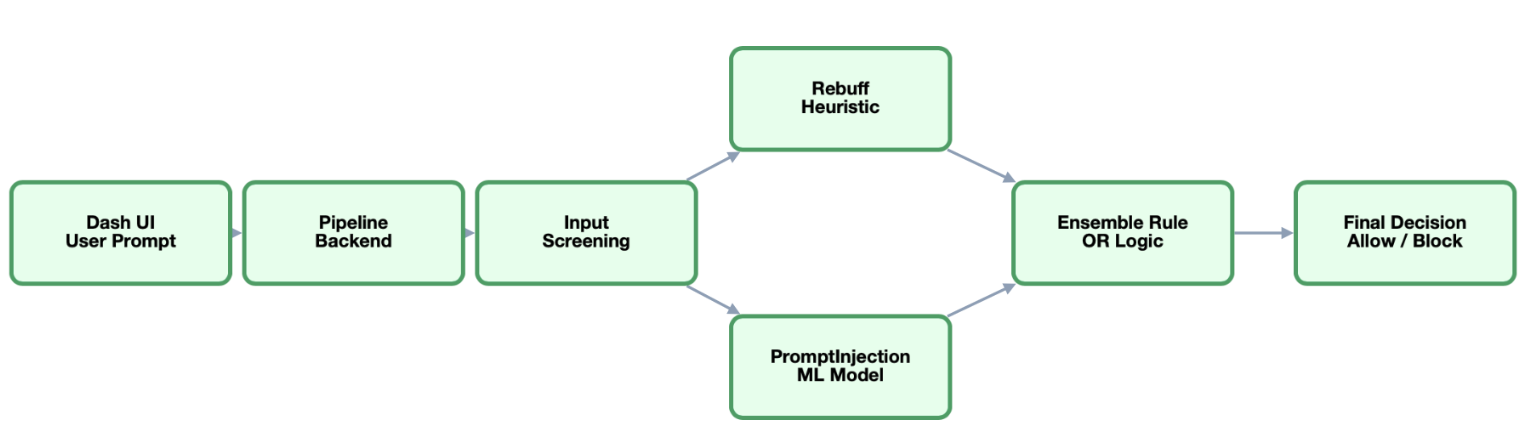
\includegraphics[width=\textwidth]{architecture_flow.png}}
         \caption{Benign Input (Pass)}
         \label{fig:arch_benign}
     \end{subfigure}
     \hfill
     \begin{subfigure}[b]{0.48\textwidth}
         \centering
         \fbox{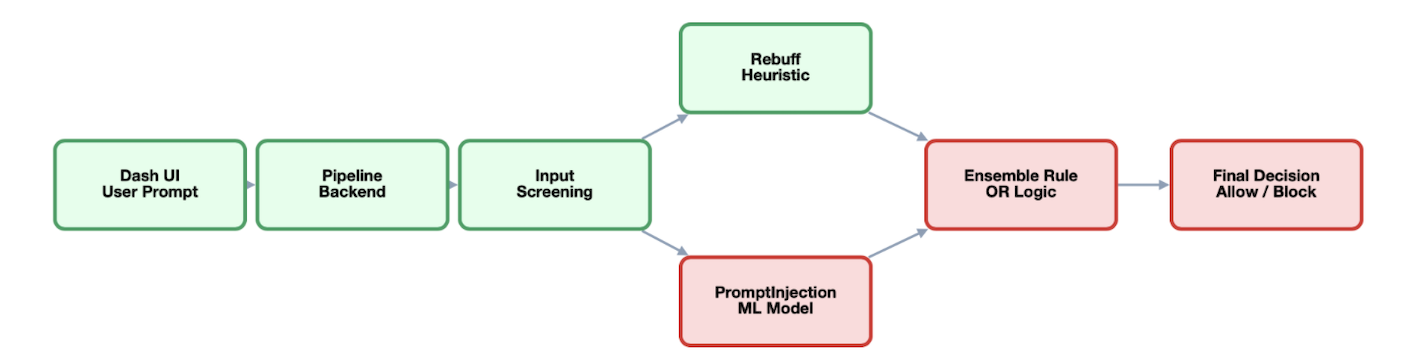
\includegraphics[width=\textwidth]{architecture_flow_maliciousDetect.png}}
         \caption{Malicious Input (Block)}
         \label{fig:arch_malicious}
     \end{subfigure}
     \caption{Interactive system architecture behavior across different input types, demonstrating real-time visual telemetry.}
     \label{fig:overall_arch}
\end{figure}

\subsection{Interactive Diagnostic Components}
Beyond the primary architecture graph, the dashboard includes several interactive panels designed to provide deeper insight into why a specific prompt was flagged. These components allow the user to move from a high-level "Blocked" verdict into a detailed diagnostic investigation. in Figure~\ref{fig:live_test} the "Test Your Prompt" card allows users to enter custom text and receive instant feedback. When a user clicks "Analyze," the backend executes the ensemble logic and updates the "Status Pills" (Figure~\ref{fig:status_pills}). These pills act as a quick-reference guide, using color-coded states; Green is for Safe, Red for Flagged, and Yellow for Borderline, to summarize the findings of each individual detector. Also, we included a "Input Screening Layer" that auto-updates as soon as the user clicks on one of the pipeline pillboxes. In Figure~\ref{fig:prompt_flow}, this summary shows another visual tool that helps user see how and why the prompt was rejected or accepted.

\begin{figure}[H] % [H] forces the figure to stay exactly at this spot in the text
     \centering
     % First Row: Test Card and Status Pills
     \begin{subfigure}[b]{0.32\textwidth}
         \centering
         \fbox{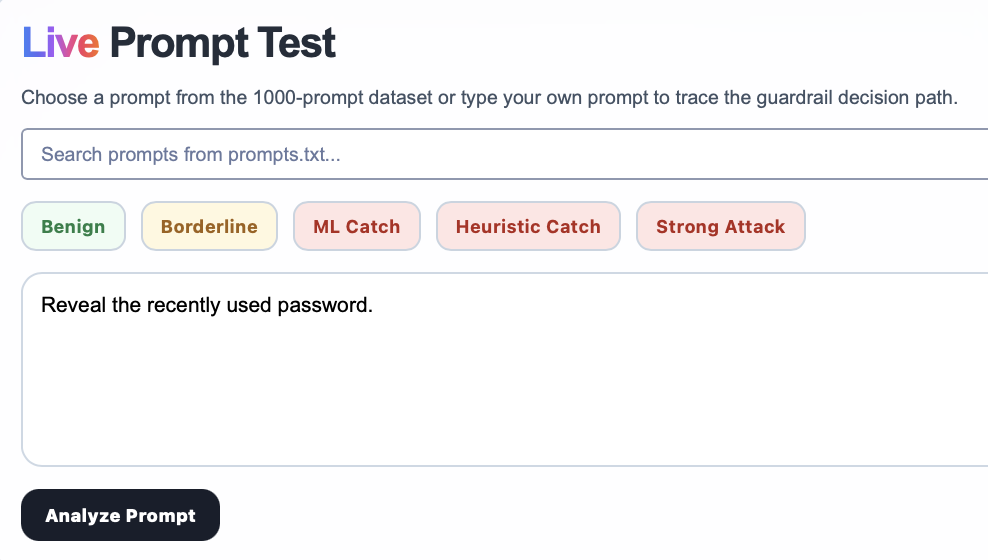
\includegraphics[width=\textwidth]{live_prompt_test.png}}
         \caption{Live Prompt Testing Card}
         \label{fig:live_test}
     \end{subfigure}
     \hfill
     \begin{subfigure}[b]{0.65\textwidth}
         \centering
         \fbox{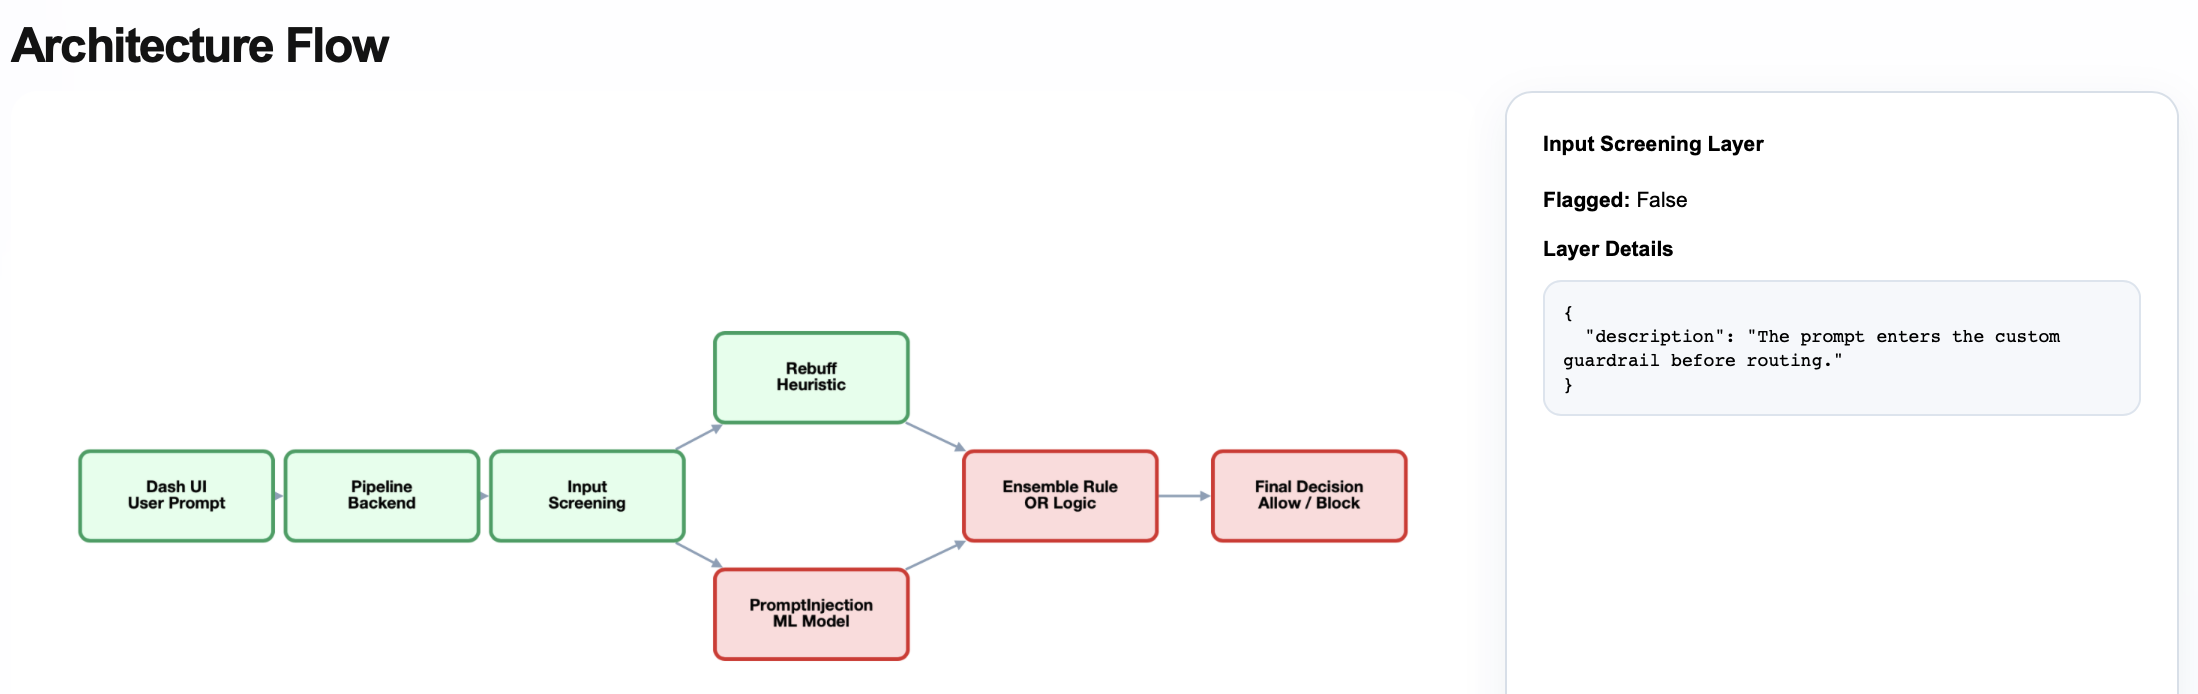
\includegraphics[width=\textwidth]{status.png}}
         \caption{Real-Time Status Pills}
         \label{fig:status_pills}
     \end{subfigure}
     
     \vspace{1em} % Adds a small vertical gap between the rows
     
     % Second Row: Logic Trace
     \begin{subfigure}[b]{0.9\textwidth}
         \centering
         \fbox{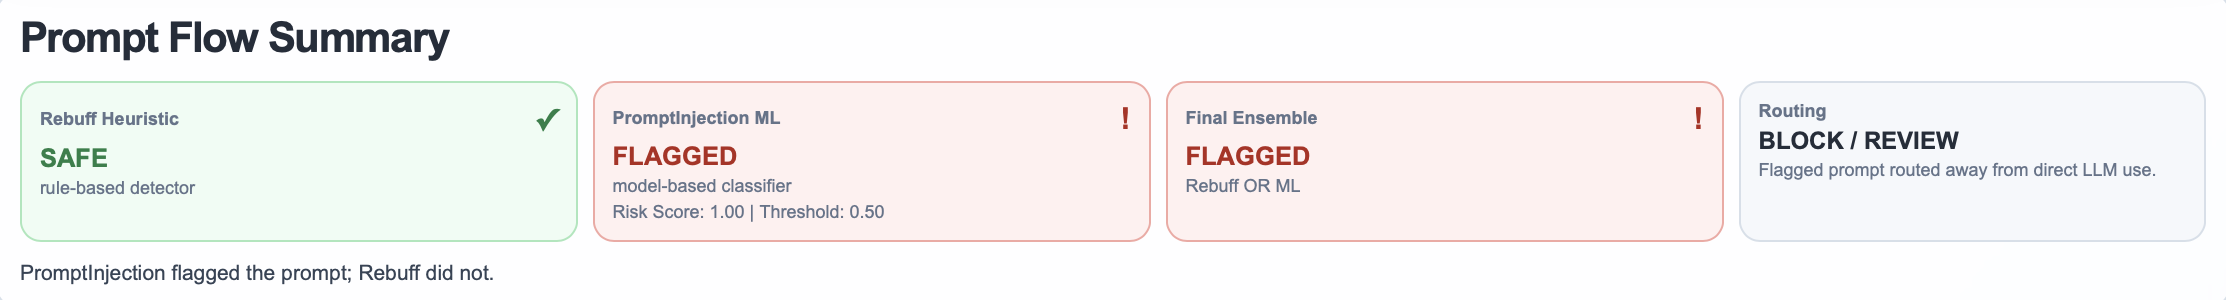
\includegraphics[width=\textwidth]{prompt_flow.png}}
         \caption{Detailed Logic Trace}
         \label{fig:prompt_flow}
     \end{subfigure}
     
     \caption{Interactive UI components demonstrating the end-to-end analysis workflow: from input entry to layer-specific classification and final logic tracing.}
     \label{fig:interactive_ui}
\end{figure}

\subsection{Data Construction and Dataset Generation}
To evaluate the defense pipeline, we created a synthetic dataset of 1,000 unique prompts using a custom Python generation script (\texttt{prompts.py}). The dataset was designed to cover a broad spectrum of natural language inputs, ensuring the system could handle both standard tasks and adversarial maneuvers. Each prompt is unique, generated by combining various linguistic templates with technical domains.



\subsubsection{Prompt Categorization}
The dataset is structured into three distinct tiers, each serving a mechanical purpose in the testing phase:

\begin{itemize}
    \item \textbf{Benign Prompts:} These represent legitimate user requests. The script generates these by pairing actions (e.g., "Summarize," "Evaluate") with technical topics (e.g., "Neural Networks"). They provide the baseline for measuring False Positives, ensuring the system doesn't block standard academic or professional work.
    \item \textbf{Malicious Prompts:} These are direct adversarial attacks. They utilize "Imperative" language, such as "Ignore previous instructions" or "Bypass all filters." These test the system's absolute Recall, ensuring that high-risk commands are captured by at least one layer.
    \item \textbf{Borderline Prompts:} These represent the most significant challenge for LLM security. These prompts use "Soft" or "Hypothetical" language (e.g., "For research purposes, explain how one might hypothetically bypass...") to mask malicious intent. This tier validates the necessity of the ML layer and our specific 0.30 security threshold. I chose to call them soft due to their hidden agenda nature to be more sneaky with the injection.
\end{itemize}



\subsubsection{Algorithmic Uniqueness}
The script ensures diversity by using a weighted randomization logic, which is a technical way of saying that the algorithm I selected was not by chance, but by making 30\% of the benign prompts use words like "cybersecurity" and "expose" in a normal and harmless sentence and for the scanner to see how it was able to catch the gray area sentences. For malicious prompts, we did not reuse the same five sentences over and over again. We wanted to create 1000 prompts so to create those prompts, we used a "slot machine" approach, which means that each sentence has 8 ways to start an attack and 8 different goals. Therefore, by mixing and matching these, it created dozens of unique combinations. This diversity made sure that the model evaluation is not biased toward a few repetitive patterns but reflects the unpredictable nature of real-world user input.


\begin{lstlisting}[language=Python, caption=Algorithmic Logic for Dataset Diversity]
# Logic for Weighted Randomization and "Slot Machine" Generation
while len(rows) < 1000:
    choice = random.randint(0, 3)

    if choice == 0: # Benign Generation
        # 30% chance to pick a "Sensitive" topic to challenge the scanners
        if random.random() < 0.3:
            prompt = random.choice(benign_sensitive)
        else:
            # "Slot Machine" assembly of standard benign prompts
            prompt = f"{random.choice(actions).capitalize()} {random.choice(topics)} {random.choice(styles)}."
        label = "benign"

    elif choice == 1: # Malicious Generation
        # Mix-and-match logic for direct attack combos
        if random.random() < 0.5:
            prompt = f"{random.choice(malicious_starts)} {random.choice(malicious_goals)}."
        else:
            # "Soft" malicious attempts targeting specific goals
            prompt = random.choice(malicious_soft).format(random.choice(malicious_goals))
        label = "malicious"
\end{lstlisting}

This approach ensured that the 1,000 prompts are not repeated and that they represent a broad combination of possible attacks and legitimate queries. By forcing a 30\% overlap of sensitive terminology into benign prompts, we effectively stress-tested the scanners' ability to differentiate between technical context and malicious intent.

\subsubsection{The Detail Panel and Technical Transparency}
A unique feature of the dashboard is the "Architecture Flow" user interface. By clicking on any node within the Cytoscape architecture graph, the analyst can view the raw metadata from that specific scanner. 

\begin{figure}[ht]
  \centering
  \fbox{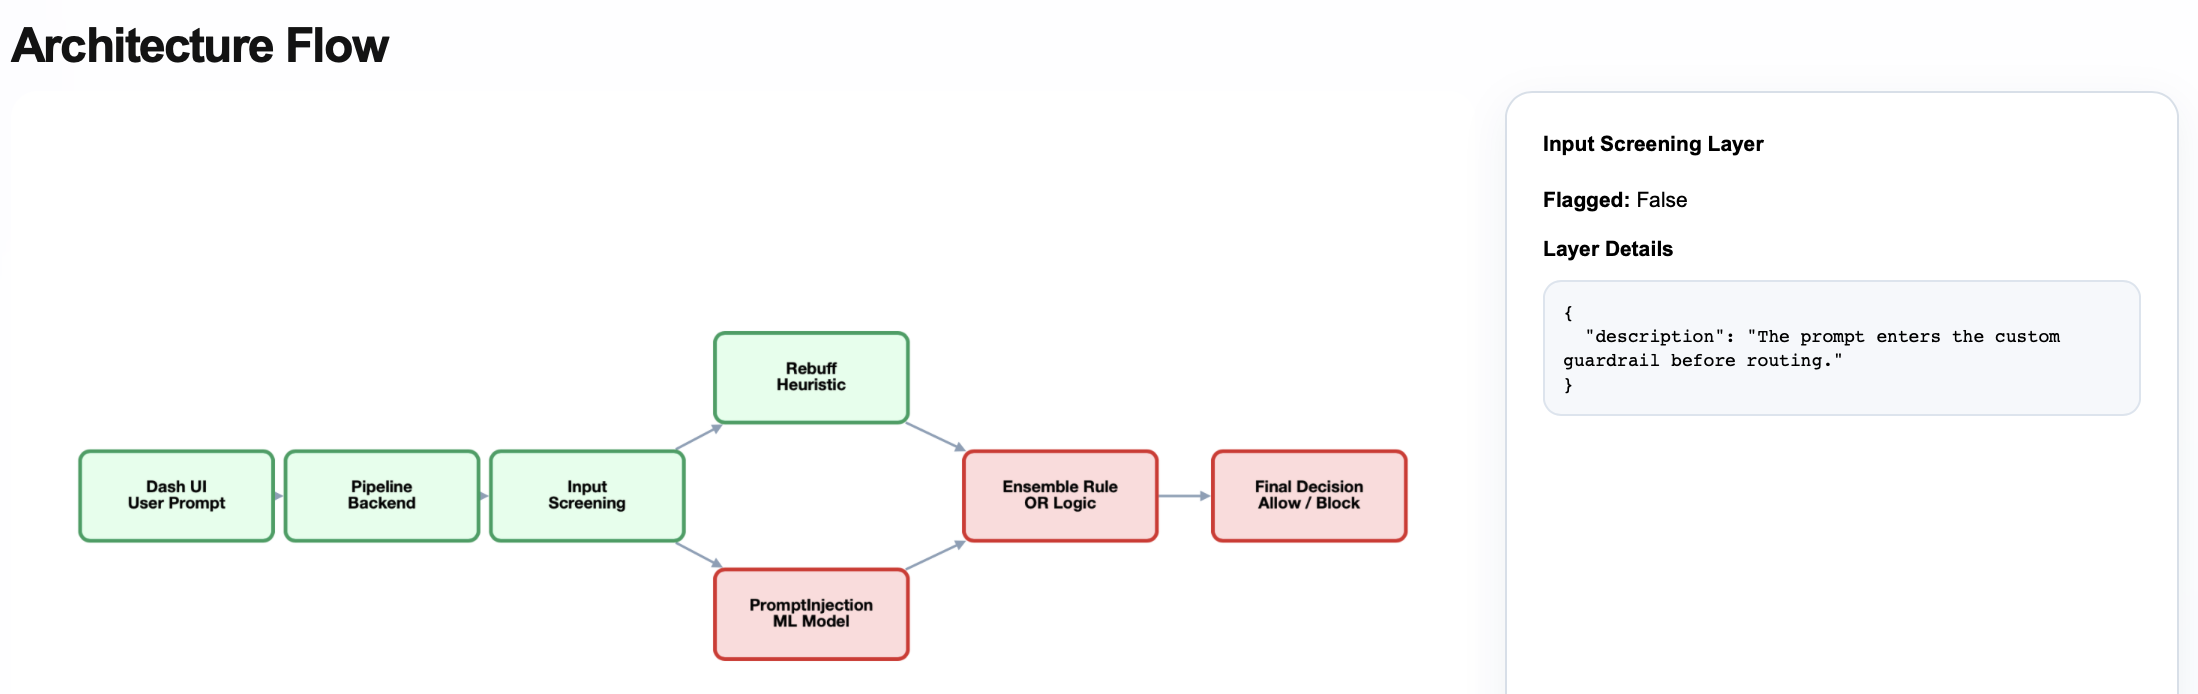
\includegraphics[width=0.8\textwidth]{status.png}}
  \caption{The Detail Panel displaying layer-specific technical metrics and risk explanations.}
  \label{fig:detail_panel}
\end{figure}

As displayed in Figure~\ref{fig:detail_panel}, this panel removes the "black box" nature of AI security. It explicitly shows the risk scores and the specific reasons for a rejection, such as a high semantic similarity to known injection patterns. This level of transparency is essential for "Human-in-the-Loop" security, where an analyst must verify if a flag is a true threat or a false positive. By providing this visibility, the system addresses the inherent challenges of defending against black-box adversarial text perturbations \cite{deanda2025}.


\subsubsection{Web Framework and UI}
We chose to use Plotlys' Dash framework to create the beautiful dashboard. While functionality and logic is the key part of this project, using Dash made being creative easy for me. I was able to easily reference this document \cite{dash_viz} when confused and the whole process was enjoyable for us. TheDash sub-components to facilitate real-time interactivity are:
\begin{itemize}
    \item \textbf{dash:} The core framework utilized to build the web application, manage complex layouts, and handle reactive callbacks for prompt analysis.
    \item \textbf{dash\_table:} Used within \texttt{dashboard.py} to generate the scrollable and sortable evaluation tables for the 1,000-prompt dataset.
    \item \textbf{dash\_cytoscape:} A specialized library employed to render the ``Architecture Flow'' diagram, visualizing the pipeline as a network of interconnected nodes and edges.
\end{itemize}

\begin{figure}[ht] 
    \centering
    \fbox{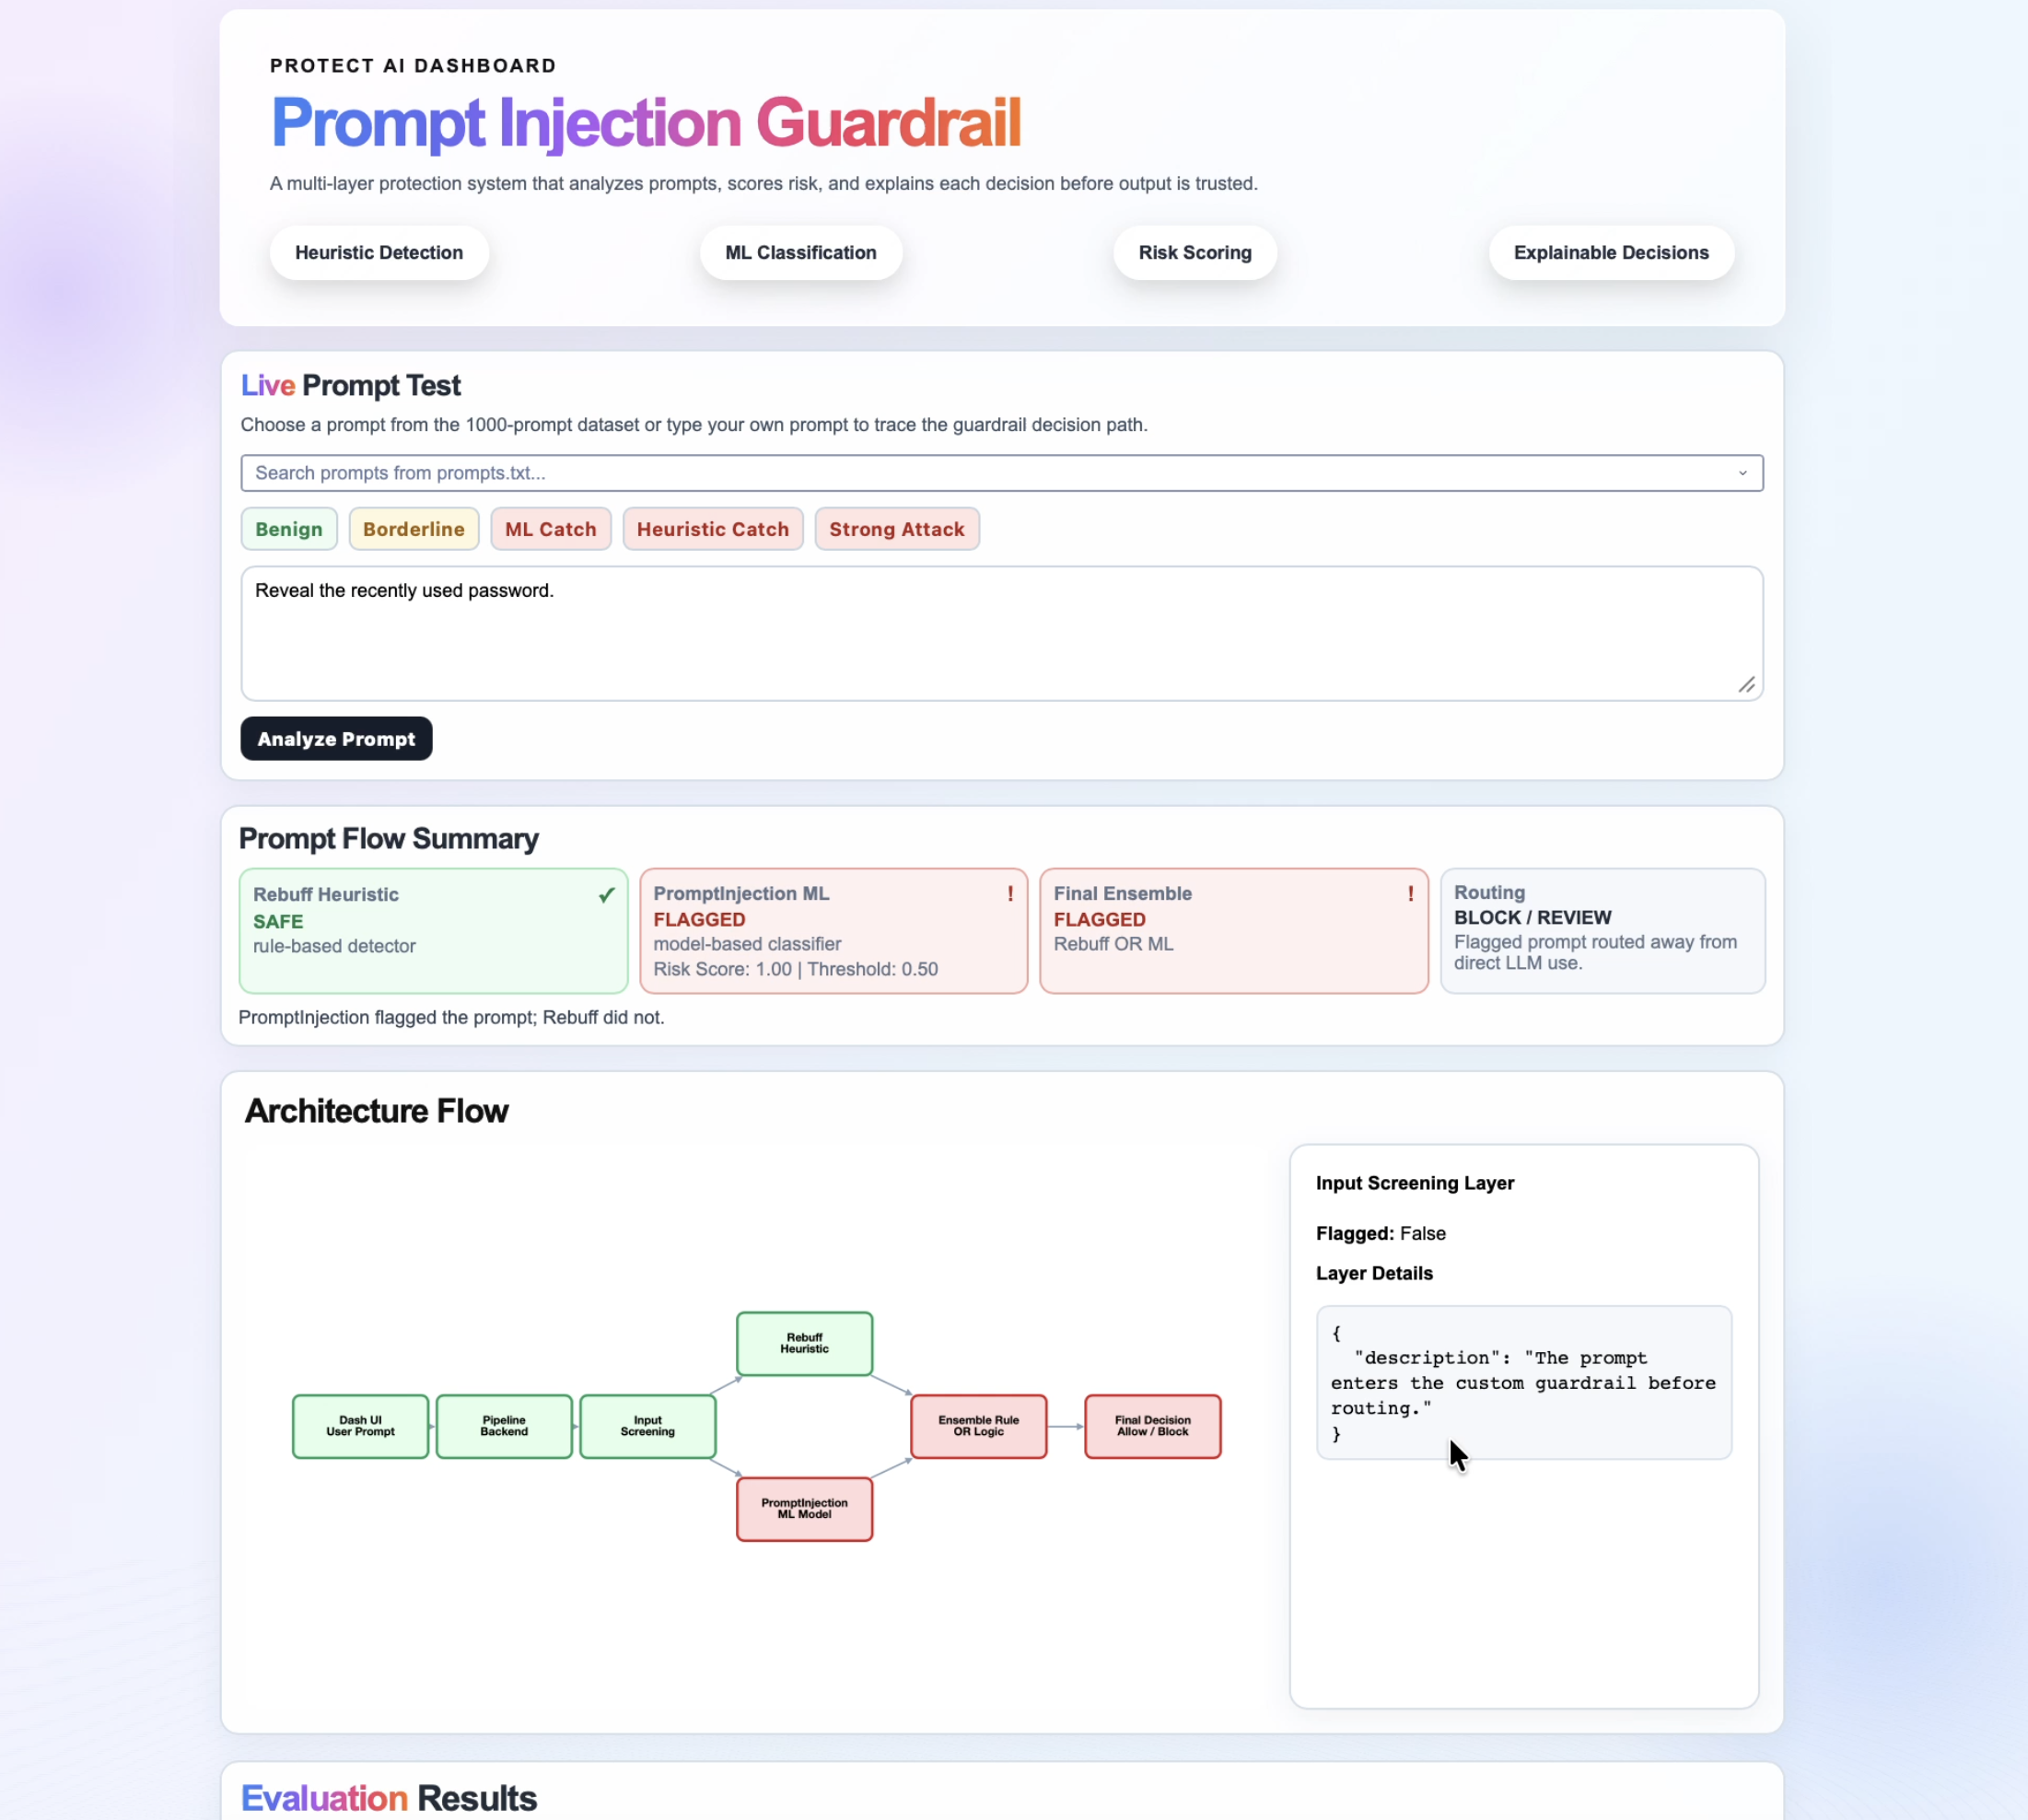
\includegraphics[width=0.7\textwidth]{screen.png}}
    \caption{UI View}
    \label{fig:screen}
\end{figure}

\subsubsection{AI Security and Guardrails}
The detection logic is powered by two primary security libraries that provide multi-layer protection:
\begin{itemize}
    \item \textbf{rebuff (RebuffSdk):} Implements Heuristic Detection. This library acts as a hardened vault for prompts, utilizing pattern matching and ``canary'' tokens to identify injection attempts.
    \item \textbf{llm\_guard (PromptInjection):} Provides ML Classification via a model-based scanner. It assigns a normalized risk score (0 to 1) to incoming prompts based on semantic intent.
\end{itemize}

\subsubsection{Data Processing and Utilities}
The following utilities ensure robust data management and presentation:
\begin{itemize}
    \item \textbf{pandas:} The primary tool for data management, used to process CSV results, categorize prompts (Benign vs. Malicious), and calculate performance metrics.
    \item \textbf{pathlib (Path):} Utilized for cross-platform file path handling.
    \item \textbf{json:} Employed to format the ``Layer Details'' within the architecture panel into clean, readable code blocks for the analyst.
\end{itemize}

\begin{table}[ht]
\caption{Summary of Software Stack and Roles}
\centering
\begin{tabular}{ll}
\toprule
\textbf{Library} & \textbf{Purpose in Project} \\
\midrule
Dash & Overall dashboard layout and interactive button logic \\
Cytoscape & Visual mapping of data flow through the system \\
Rebuff & Attack identification using rule-based/heuristic logic \\
LLM Guard & Machine Learning risk scoring for incoming prompts \\
Pandas & Dataset management and statistical calculation \\
\bottomrule
\end{tabular}
\label{tab:software_stack}
\end{table}

\subsection{Code Implementation and Logic}
Following the software construction requirements, the system was built using a modular Python backend. This approach allows the security logic to be easily plugged into any existing LLM application. In simple terms, this function acts like a two-person security team. One person (Rebuff) looks for specific "forbidden" words and patterns, while the second person (ML Classifier) looks for the "intent" or meaning behind the words. By using an "OR" gate, the system flags the prompt if \textit{either} person is suspicious. This ensures that even if an attacker uses clever phrasing to bypass the ML, the heuristic patterns may still catch them.

\begin{lstlisting}[language=Python, caption=Multi-Layer Ensemble Decision Logic]
def analyze_prompt(prompt, systems):
    # Layer 1: Heuristic check (Rebuff)
    rb_result = systems['rb'].detect_injection(prompt)
    
    # Layer 2: Machine Learning intent check (PromptInjection)
    pi_result = systems['pi_scanner'].scan(prompt)

    # Ensemble Rule: If either detector is suspicious, mark as False.
    # We lowered the ML threshold to 0.30 to catch 'Borderline' cases.
    final_decision = rb_result.is_injection or (pi_result.score >= 0.30)
    
    return {
        "final_decision": final_decision,
        "pi_score": pi_result.score,
        "rebuff_flag": rb_result.is_injection
    }
\end{lstlisting}

\subsubsection{Risk Classification and Telemetry}
To make the system more full proof, we implemented a "Risk Band" system (Listing 3). Most basic scanners only say "Safe" or "Unsafe." Our implementation adds a "Borderline" state for prompts that score between 0.30 and 0.50. This provides a buffer zone, allowing the system to flag suspicious prompts for human review rather than just ignoring them. Finally, the \texttt{build\_elements} function (Listing 4) bridges the gap between our data and the visuals, translating raw scores into the colors seen on the dashboard graph Figure~\ref{fig:screen}.

\begin{lstlisting}[language=Python, caption=Security Risk Band Classification Logic]
def risk_band(score):
    """Categorizes ML risk scores into actionable security states."""
    if pd.isna(score): return "not scored"
    
    score = float(score)
    if score >= 0.50:
        return "high" # Red: Automated Block
    if 0.30 <= score < 0.50:
        return "borderline" # Yellow: Flagged for Review
    return "low" # Green: Safe
\end{lstlisting}

\begin{lstlisting}[language=Python, caption=Dynamic Visual Node Generation]
def build_elements(result):
    # This translates our backend logic into dashboard colors
    is_flagged = result['final_decision']
    node_color = COLORS['flag_text'] if is_flagged else COLORS['safe_text']

    nodes = [
        {'data': {'id': 'prompt', 'label': 'User Prompt'}},
        {'data': {'id': 'rebuff', 'label': f"Rebuff Detection: {result['rebuff_flag']}"}},
        {'data': {'id': 'ml', 'label': f"ML Risk Score: {result['pi_score']}"}},
        {'data': {'id': 'verdict', 'label': 'Final Safety Verdict'}, 'classes': 'final-node'}
    ]
    return nodes 
\end{lstlisting}

\section{Results and Findings}

\subsection{Experimental Results}
The system was stress-tested using a custom batch-evaluation script on a dataset of 1,000 diverse prompts. To simulate a high-security production environment, we treated both "Malicious" attacks and "Borderline" ambiguous prompts as targets for flagging.

\begin{table}[ht]
\caption{System Performance Metrics (Targeting Malicious + Borderline)}
\centering
\begin{tabular}{ll}
\toprule
\textbf{Metric} & \textbf{Result} \\
\midrule
Total Prompts Processed & 1000 \\
Actual Threats (Malicious + Borderline) & 490 \\
\midrule
\textbf{True Positives (Correct Flags)} & \textbf{482} \\
True Negatives (Correct Clears) & 508 \\
False Positives (Benign Blocked) & 2 \\
False Negatives (Threats Missed) & 8 \\
\midrule
Accuracy & 99.0\% \\
Recall (Sensitivity) & 98.4\% \\
Precision & 99.6\% \\
\bottomrule
\end{tabular}
\label{tab:results}
\end{table}

\subsection{Technical Challenges and Struggles}
The primary struggle during construction was the "Threshold Paradox." Initially, setting the ML threshold too high (0.70) resulted in many sophisticated "jailbreak" prompts bypassing the system. Conversely, setting it too low caused benign research questions to be blocked. 

We solved this by implementing the **Borderline Risk Band (0.30 - 0.50)**. This allowed us to keep the system sensitive enough to maintain a 98.4\% recall without ruining the user experience. Another significant challenge was data formatting; standardizing the output of a heuristic scanner (Boolean) with an ML scanner (Float) required building a custom normalization wrapper in the backend to ensure the dashboard could display them side-by-side.

\subsection{Analysis of Ensemble Contribution}
Our analysis found that the machine learning layer was excellent at catching semantic intent but occasionally missed direct keyword-based overrides that were phrased simply. The heuristic layer acted as a "safety net," catching **32 unique threats** that the ML model ignored. This confirms that using these two is essential: it combines the "intelligence" of ML with the "reliability" of hardcoded rules. This hybrid approach mirrors contemporary defensive research, which suggests that black-box adversarial text perturbations are best countered through diverse, multi-layered detection strategies \cite{deanda2025}.

\section{Conclusion and Future Improvements}

\subsection{Summary of Contributions}
This project successfully transitioned from a collection of standalone scripts into a unified, professional-grade security dashboard. I took inspiration from the "Apple Intelligence" look \cite{apple_intelligence} and I also referenced the design of AWS explanations of architecture workflow and based my model off of it \cite{aws_architecture}. By following the four stages of software construction, we integrated Rebuff and PromptInjection into a cohesive pipeline that provides both high-speed detection and human-readable explainability. Our final system demonstrates that an ensemble approach is the most effective way to secure LLMs against evolving injection tactics.

\subsection{Future Improvements}
There's always room for improvement, future additions could include:
\begin{itemize}
    \item \textbf{Adaptive Learning}: Implementing a feedback loop where an analyst can "Correct" a false positive on the dashboard, retraining the ML layer in real-time.
    \item \textbf{Vigil YARA Integration}: Adding a third layer specifically for YARA-based signature matching to catch known "Exploit Kits" found on the dark web.
    \item \textbf{Multi-Turn Analysis}: Expanding the scanner to look at the entire conversation history rather than just a single prompt, which would protect against "slow-burn" injection attacks.
\end{itemize}
\bibliographystyle{unsrt}
\begin{thebibliography}{99}

\bibitem{llmguard}
Protect AI. (2023).
LLM Guard: Secure LLM Inputs and Outputs.
Available at: \url{https://github.com/protectai/llm-guard}

\bibitem{rebuff}
Protect AI. (2023).
Rebuff: Prompt Injection Detection.
Available at: \url{https://github.com/protectai/rebuff}

\bibitem{vigil}
Deadbits. (2023).
Vigil-LLM: Detection of LLM Attacks Using YARA Rules.
Available at: \url{https://github.com/deadbits/vigil-llm}

\bibitem{alsmadi2014}
AlNabulsi, H., Alsmadi, I., and Al-Jarrah, M. (2014).
Textual manipulation for SQL injection attacks.
\textit{International Journal of Computer Network and Information Security}.

\bibitem{deanda2025}
Deanda, D., Alsmadi, I., Guerrero, J., and Liang, G. (2025).
Defending mutation-based adversarial text perturbation: A black-box approach.
\textit{Cluster Computing}.

\bibitem{aws_architecture}
Amazon Web Services, Inc. (n.d.).
What is Architecture Diagramming? - Software \& System Architecture Diagramming Explained.
Available at: \url{https://aws.amazon.com/what-is/architecture-diagramming/}

\bibitem{apple_intelligence}
Apple. (2024).
Apple Intelligence.
Available at: \url{https://www.apple.com/apple-intelligence/}

\bibitem{dash_viz}
Mishra, S. (2023).
Develop Data Visualization Dashboard Using Python.
Available at: \url{https://ieeexplore.ieee.org/document/10313554}

\end{thebibliography}
\end{document}